\section{Event generation for inclusive DIS}
\label{sec:inclusive}
\label{sec:results}

We consider first the results of event generator benchmarking for inclusive DIS, where only the fiducial cuts of Eq.~(\ref{eq:fiducial}) are applied, and compare predictions both for total cross-sections and for differential distributions in the DIS kinematic variables.
%
In the following sections we consider charm-tagged cross-sections (Sect.~\ref{sec:charm}), observables dependent on the final-state hadronic system at the level of the FASER$\nu$ acceptance (Sect.~\ref{sec:hadronic}), and the Tier S and dimuon selections in the applications to FASER (Sect.~\ref{sec:faser-app}). 

\paragraph{Total fiducial cross-sections.}
\label{sec:incl-nlo}
\label{sec:incl-scales}
%
Fig.~\ref{fig:sigma-vs-energy} displays the inclusive fiducial cross section (evaluated per nucleon) on a tungsten target as a function of the beam energy for muon $(\mu^-)$ neutral-current and muon-neutrino ($\nu_\mu$) charged-current DIS.
%
This fiducial region is defined by $Q^2 > 4$~GeV$^2$ and $W > 3$~GeV, Eq.~(\ref{eq:fiducial}).
%
We provide results for three NLO-matched event generators (\sherpa, \herwig, and \powhegres for neutral-current or \powhegtwo for charged-current scattering) as well as for the analytical structure-function calculations from \yadism at NLO and NNLO.
%
MHOUs are evaluated from \yadism both at NLO and at NNLO.
%
At NLO, \yadism predictions are provided in the ZM-VFNS and FONLL schemes, so that their difference estimates the impact of charm mass effects in the total cross-section.
%
At NNLO, we use FONLL for neutral-current and ZM-VFNS for charged-current scattering, since in the latter case the massive coefficient functions, although known at NNLO~\cite{Berger:2016inr,Gao:2017kkx,Caola:2026kvl}, are not implemented in \yadism. 
%
The bottom panels display the ratio of the various calculations to the 
    massless NLO \yadism calculation.

%%%%%%%%%%%%%%%%%%%%%%%%%%%%%%%%%%%%
\begin{figure}[!tbp]
  \centering
  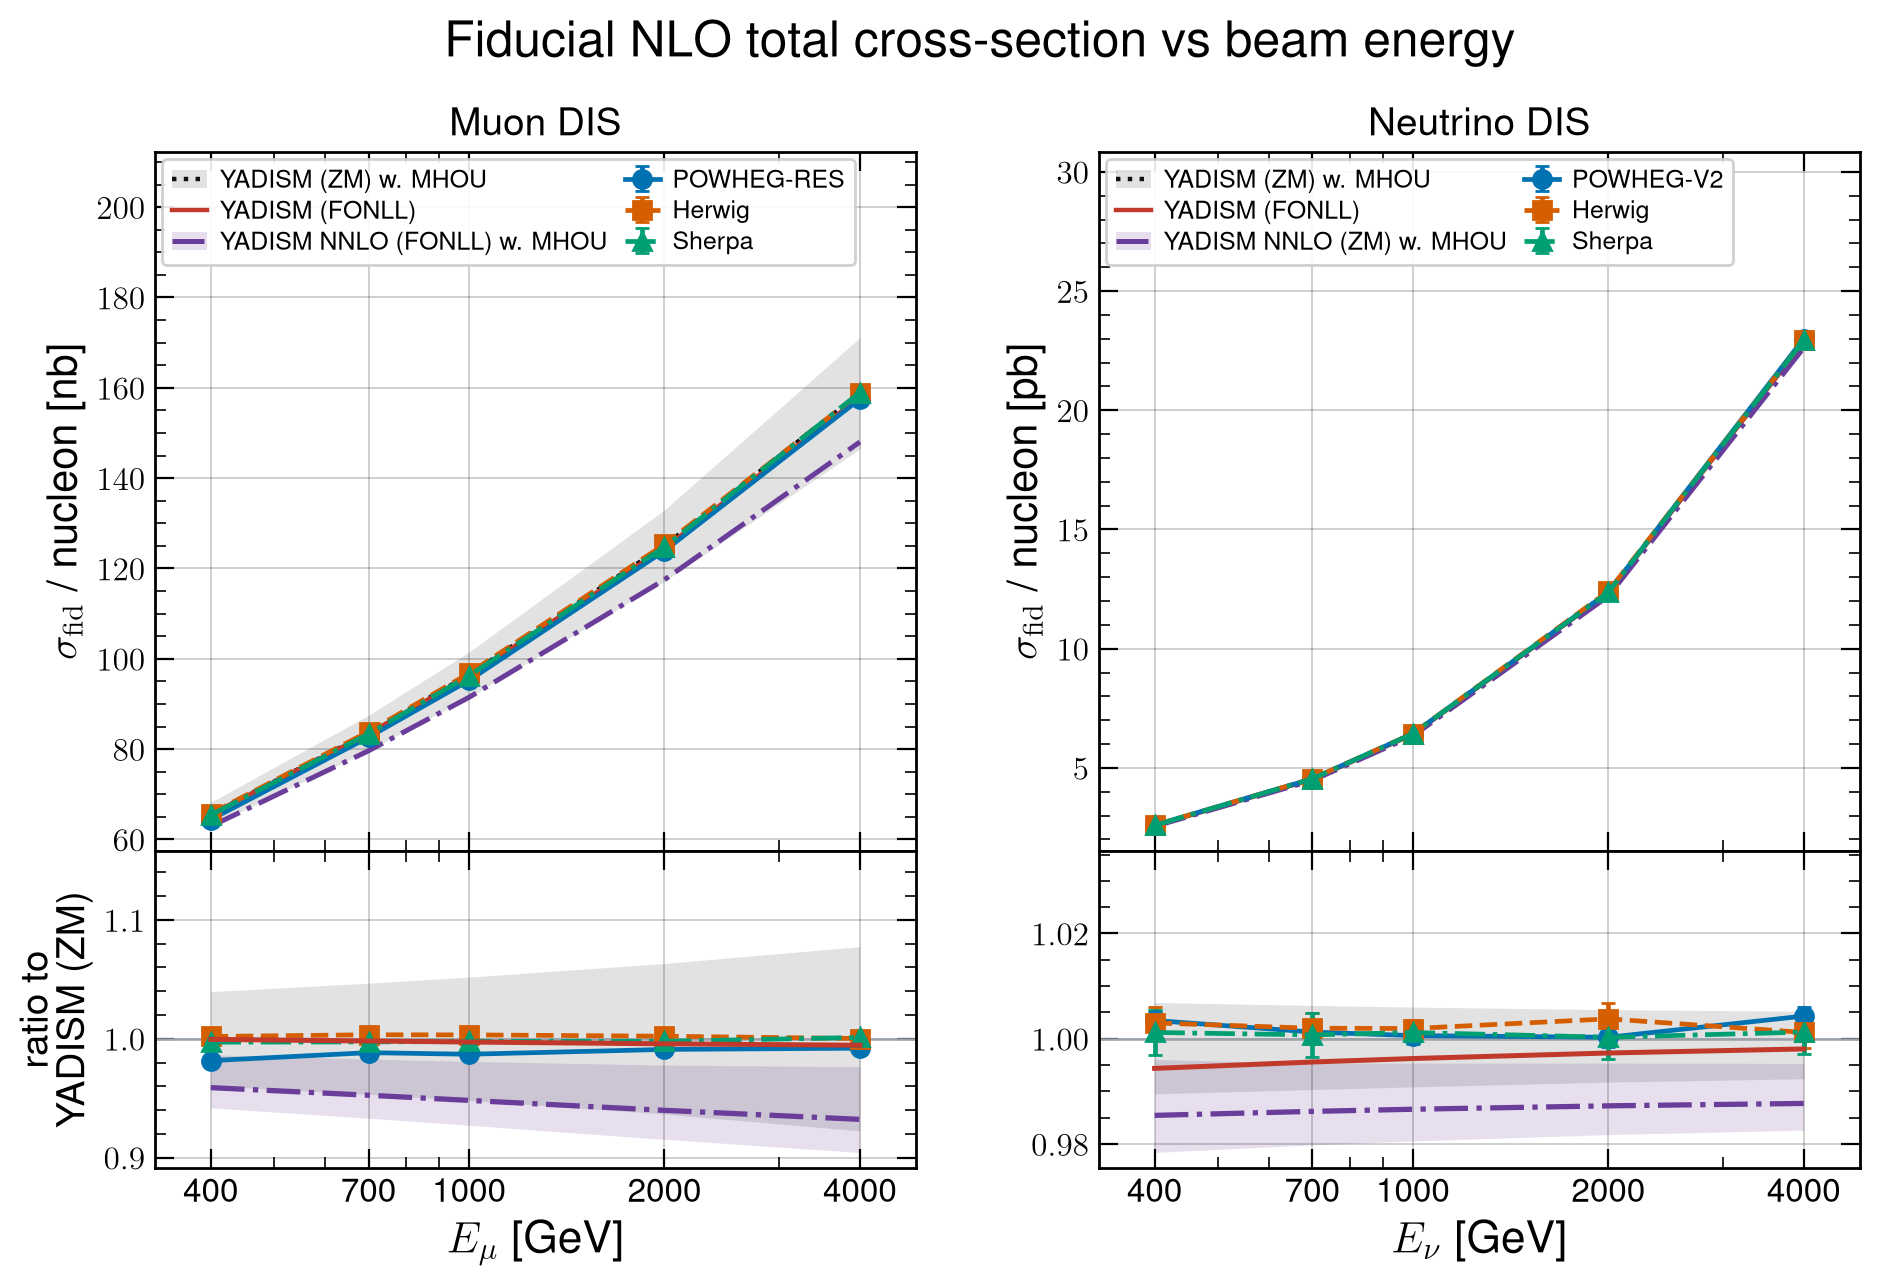
\includegraphics[width=0.98\textwidth]{figures/pp_sigma_vs_energy.png}
  \caption{Inclusive fiducial cross section per nucleon on a tungsten target as a function of the beam energy for muon $(\mu^-)$ neutral-current (left) and muon-neutrino ($\nu_\mu$) charged-current (right) scattering.
%
The fiducial region is defined by $Q^2 > 4$~GeV$^2$ and $W > 3$~GeV.
%
We provide results for three NLO-matched event generators (\sherpa, \herwig, and \powhegres or \powhegtwo) as well as for the analytical structure-function calculations from \yadism at NLO and NNLO, including the associated MHOU estimate from the latter. 
%
The bottom panels display the ratio of the various calculations to the 
    massless \yadism calculation.
%
See text for more details. 
    }
  \label{fig:sigma-vs-energy}
\end{figure}
%%%%%%%%%%%%%%%%%%%%%%%%%%%%%%%%%%%

The total fiducial rates predicted by the three NLO-matched generators agree among themselves and with the \yadism reference at the $\lsim 2\%$ level. 
%
NNLO corrections range between $-4\%$ and $-7\%$ for muon DIS and are around $-1.5\%$ for neutrino DIS; for both currents the NLO and NNLO MHOU bands overlap.
%
The fact that MHOUs are larger for NC as compared to CC is partially explained by the fact that the former probe smaller values of $Q^2$ due to the $Q^{-4}$ enhancement of the virtual photon propagator. 
%
We have checked that raising the momentum-transfer cut in $Q^2$ markedly reduces the MHOUs in neutral-current DIS.
%
Furthermore, charm mass effects, as estimated by the \yadism FONLL calculation, are negligible at the level of inclusive fiducial cross-sections. 
%
The agreement between the three generators and the \yadism reference shown in Fig.~\ref{fig:sigma-vs-energy}, despite the use of different parton shower algorithms and hadronisation models, confirms that fiducial cross-sections are, as expected, determined by the DIS matrix elements, which are identical in all the massless NLO calculations shown.

\paragraph{Differential distributions.}
\label{sec:incl-diff}
%
Fig.~\ref{fig:dis-distributions} displays the same benchmark comparison between the predictions of NLO-matched event generators and analytical structure function calculations as in Fig.~\ref{fig:sigma-vs-energy},  now for differential distributions in the same fiducial region.
%
For illustration purposes we show $E_\ell=1$ TeV as
representative energy; we have verified that the results are qualitatively similar at other incoming lepton energies.
%
As in Fig.~\ref{fig:sigma-vs-energy}, we quote the differential cross-sections per nucleon on a tungsten target, and their integral reproduces the values indicated in Fig.~\ref{fig:sigma-vs-energy}.
%
Error bars in the generator predictions are the  Monte Carlo integration statistics in each case.
%
The bottom panels show the ratio to the NLO massless \yadism reference calculation.

From top to bottom, we show the distributions in Bjorken $x_{\rm Bj}$, the scattered-lepton energy $E_{\ell'}$ and polar angle $\theta_{\ell'}$, and the momentum transfer $Q^2$, in all cases in the target rest frame.
%
Note that these distributions are not all independent, since for a fixed beam energy the scattering kinematics only has two degrees of freedom.
%
For instance, $Q^2 = 2 E_\ell E_{\ell'} (1 - \cos\theta_{\ell'})$.
%
Furthermore, the hadronic energy $E_h$ and inelasticity $y$ are not shown, since for fixed $E_\ell$ they are both linear in $E_{\ell'}$, hence comparing the different calculations for the latter is sufficient. 
%
These are observables that the  analytic calculation can predict, since they are built from the leptonic kinematics without reference to the hadronic final state.

%%%%%%%%%%%%%%%%%%%%%%%%%%%%%
\begin{figure}[!tbp]
  \centering
  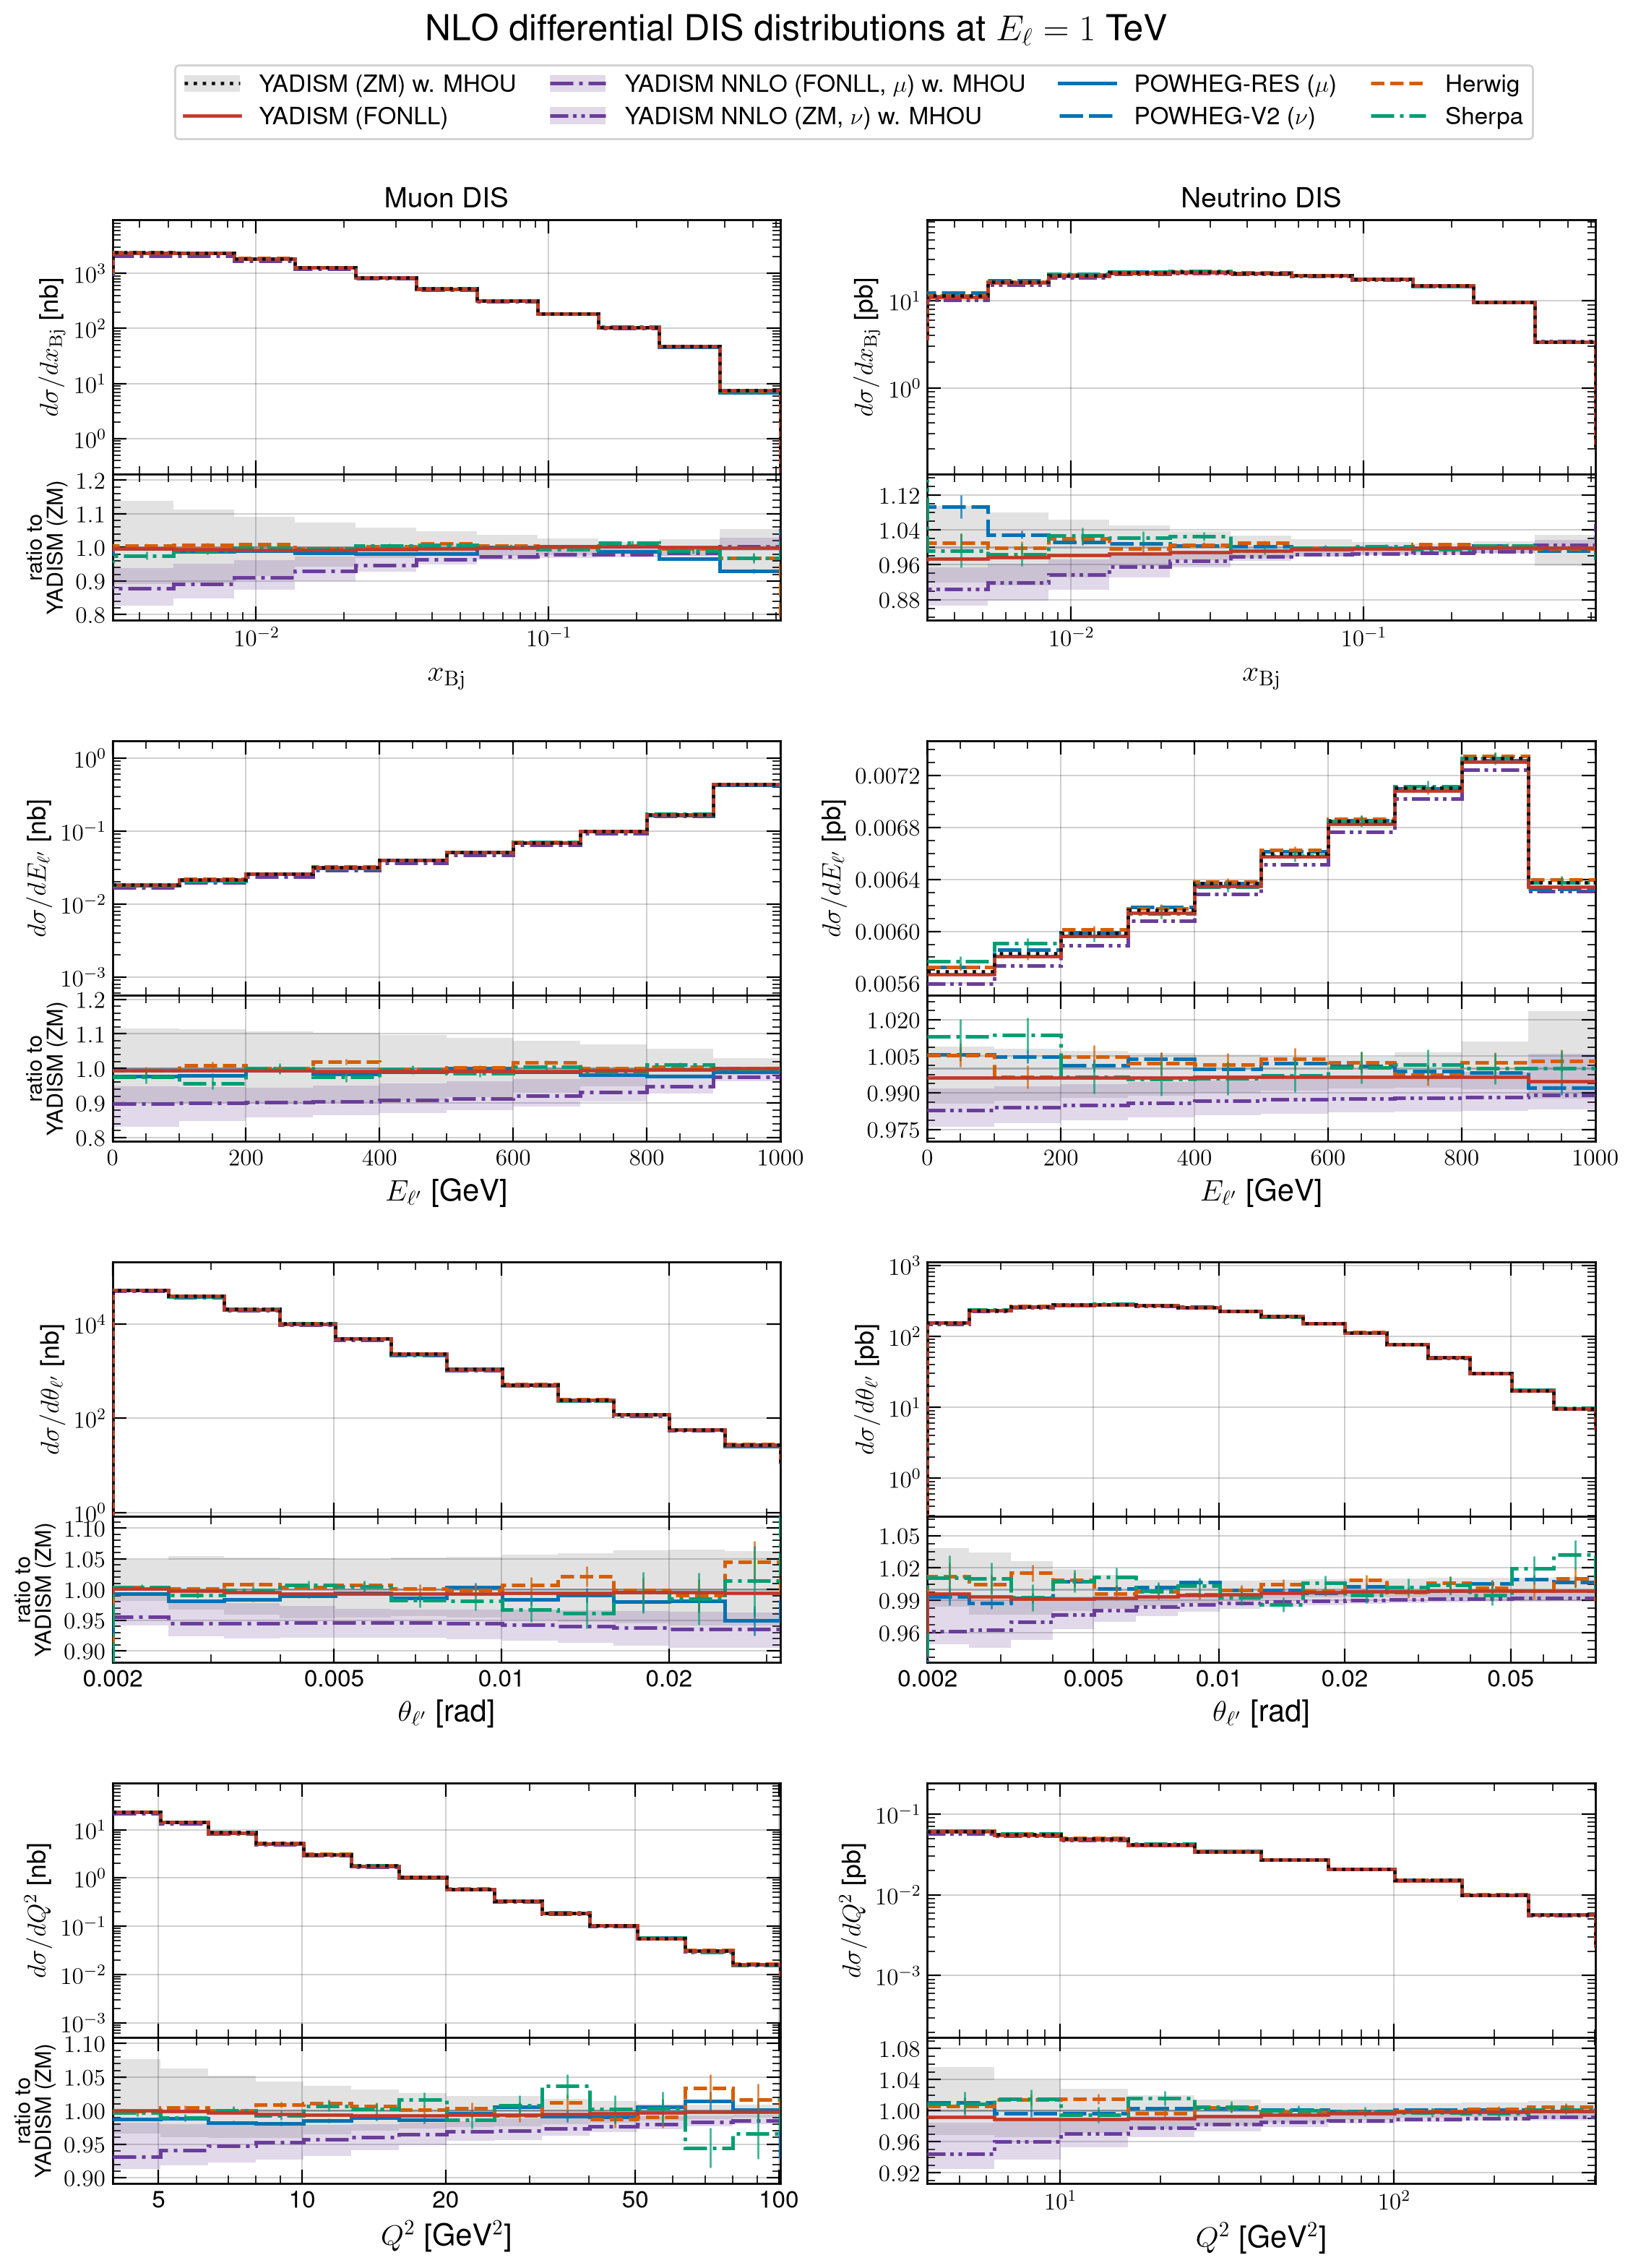
\includegraphics[width=0.96\textwidth]{figures/pp_dis_distributions.png}
  \caption{Same as Fig.~\ref{fig:sigma-vs-energy}, namely the cross-sections per nucleon on a tungsten target, for differential distributions in the fiducial region at the representative energy of $E_\ell=1$ TeV.
%
From top to bottom, we show the distributions in Bjorken $x_{\rm Bj}$, the scattered-lepton
    energy $E_{\ell'}$ and polar angle $\theta_{\ell'}$, and the momentum transfer $Q^2$, in all cases in the target rest frame.
    %
    Error bars in the generator predictions are the  Monte Carlo integration statistics in each case.}
  \label{fig:dis-distributions}
\end{figure}
%%%%%%%%%%%%%%%%%%%%%%%%%%%%%%%

The main result of Fig.~\ref{fig:dis-distributions} is the excellent agreement between the NLO generators and the analytical \yadism (ZM-VFNS) reference for both currents, echoing the agreement at the  integrated cross section level.
%
Residual differences are at the per-cent level, at most 2\% in the median bin, with individual bins deviating by up to 9\% at the lowest values of $x_{\rm Bj}$.
%
These differences between event generators and \yadism (ZM-VFNS) are overwhelmingly covered by the NLO MHOU band. 
%
As for the fiducial cross-sections, this agreement is reassuring since the displayed distributions should not be sensitive to the modelling of the hadronic final state and depend only on the NLO partonic matrix element (all other physical inputs kept the same).

From Fig.~\ref{fig:dis-distributions} we also find that, as was the case for inclusive cross-sections, NNLO corrections can be sizeable for muon DIS across the whole phase space.
%
For charged-current scattering, NNLO corrections can be considerably larger than at the inclusive level, reaching for example $-10\%$ at small $x_{\rm Bj}$ and $-6\%$ at small $Q^2$.
%
This result strengthens the need for DIS event generators reaching NNLO accuracy to ensure the full scientific exploitation of the FASER and SND@LHC far-forward physics programme.
%
Charm-mass effects, on the other hand, remain negligible also at the level of differential distributions. 
%
Indeed, charm-mass effects remain
below $3\%$ in every bin, smaller than the spread between generators.

Having established that three NLO-matched event generators agree with the structure-function calculation for a common set of physics settings, we move to discuss the comparison with \genie, the baseline generator used in FASER.
%
Here we keep this comparison at the level of inclusive and differential DIS observables in the fiducial region Eq.~(\ref{eq:fiducial}), and in Sect.~\ref{sec:hadronic} we revisit the comparison for observables at the level of the FASER$\nu$ selection.

\paragraph{Comparison with \genie.}
%
Fig.~\ref{fig:genie-vs-energy} displays, in the same format as Fig.~\ref{fig:sigma-vs-energy}, a comparison of the total inclusive cross-sections predicted by \yadism NLO in the FONLL general-mass scheme with \powhegres (muon DIS) and \powhegtwo (neutrino DIS) and different \genie tunes.
 %
 In the left panel, we show predictions with \genie {\tt G18\_02a} tune at LO matrix elements and GRV98LO and NNPDF4.0 NNLO as PDF sets.
 %
 In the right panel, we show the same LO tune and in addition the NLO {\tt GHE19\_00a} tune with {\sc\small HEDIS}, which evaluates NLO structure functions with \apfel. 
  %
  The lower panels display the ratio to the \yadism FONLL reference.
  %
  In all panels, the \yadism MHOUs are displayed.
  %
  For the case of the {\tt G18\_02a} tune we stop the energy scan at $E_\ell=1$ TeV, its declared limit of validity. 
%
The {\tt G18\_02a} tune of \genie with GRV98 LO as input PDF is the current baseline calculation used in FASER data analysis. 
%
We use \yadism FONLL as reference since this \genie cross-section model also accounts for the charm mass effects. 

%%%%%%%%%%%%%%%%%%%%%%%%
\begin{figure}[!tbp]
  \centering
  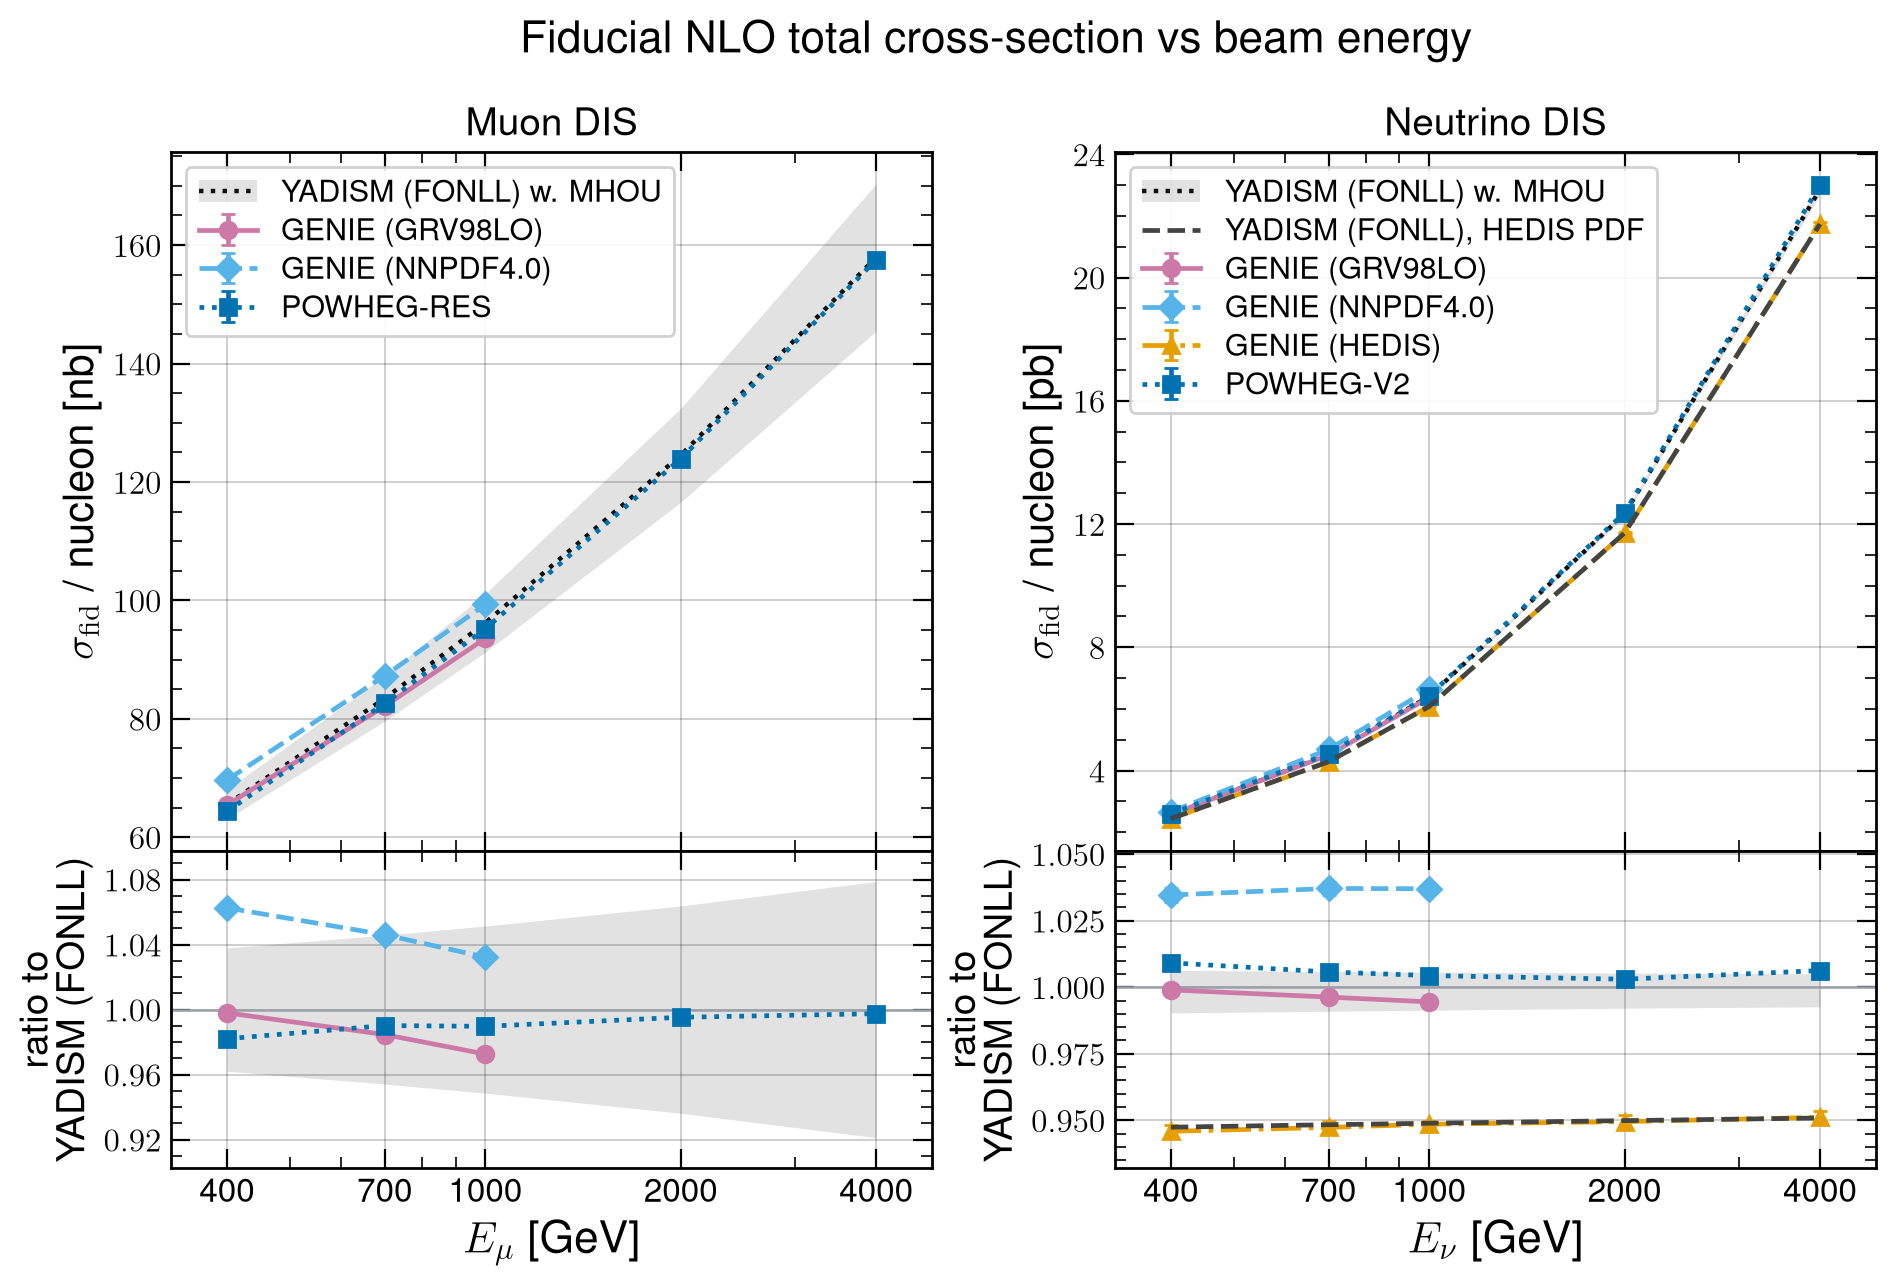
\includegraphics[width=0.98\textwidth]{figures/pp_genie_vs_energy.png}
  \caption{Same as Fig.~\ref{fig:sigma-vs-energy}
 comparing the total inclusive cross-sections predicted by \yadism NLO in the FONLL scheme with \powhegres (muon DIS) and \powhegtwo (neutrino DIS) and different \genie tunes: GRV98 (default), same with NNPDF4.0, and the {\sc\small HEDIS} tune. 
  %
  In the right panel we also display the  \yadism FONLL prediction evaluated with the same PDF set that {\sc\small HEDIS} uses, namely {\tt NNPDF31sx\_nlo\_as\_0118\_LHCb\_nf\_6}.
  %
  The lower panels display the ratio to the \yadism reference.
  %
  For the case of the default \genie tune we stop the energy scan at $E_\ell=1$ TeV, its declared limit of validity. 
 }
  \label{fig:genie-vs-energy}
\end{figure}
%%%%%%%%%%%%%%%%%%%%%%%%%%%%%%%%%%%%

From Fig.~\ref{fig:genie-vs-energy} we observe that the default \genie tune agrees with both NLO calculations (\yadism and \powheg) due to an accidental cancellation of competing effects (PDF and matrix element models).
%
For muon DIS, the use of the same PDF set (NNPDF4.0) results in a cross-section up to 6\% higher than the \yadism NLO reference.
%
For neutrino DIS a similar effect is found, and there the NLO tune based on {\sc\small HEDIS} predicts a suppression of the inclusive rates by 5\% in the considered $E_\nu$ range.
%
This last offset is entirely a PDF effect, and Fig.~\ref{fig:genie-vs-energy} shows it directly: {\tt GHE19\_00a} evaluates its structure functions with {\tt NNPDF31sx\_nlo\_as\_0118\_LHCb\_nf\_6}~\cite{Ball:2017otu,Bertone:2018dse,NNPDF:2017mvq}, whose light-quark densities lie $4$--$8\%$ below those of \nnpdf over the range $0.02 < x < 0.5$ that carries the rate.
%
The dashed grey curve is the same \yadism FONLL reference evaluated with that set, and the {\sc\small HEDIS} points lie on it: the two NLO calculations agree to $0.2\%$ at every energy and to $0.04\%$ from $E_\nu=1$~TeV up, within the statistical uncertainty of the \genie sample itself.
%
Neither the perturbative order, which is NLO on both sides, nor $\alpha_s$, which {\sc\small HEDIS} takes from its own PDF at the same value, nor the heavy-quark masses, nor the target-mass corrections contribute at this level.
%
From this assessment one can infer that while the default tune of \genie reproduces the predictions of NLO QCD calculations with modern PDFs, there is no guarantee this agreement extends to differential observables due to its accidental nature.

To illustrate this,  Fig.~\ref{fig:genie-dis-distributions} compares the DIS differential distributions ($x_{\rm Bj}, E_{\ell'}, \theta_{\ell'}$, and $Q^2$) at $E_\ell=1$ TeV between \yadism NLO, \powheg, and the same \genie tunes as those shown in Fig.~\ref{fig:genie-vs-energy}.
%
As opposed to the inclusive case, indeed now differences between the default \genie tune (with GRV98LO as input PDFs) and the NLO QCD calculations (\yadism and \powheg, which agree with each other for all observables) can be significant.
%
For example, between $-16\%$ and $+22\%$ ($-15\%$ and $+8\%$) for the $x_{\rm Bj}$ distribution in muon (neutrino) DIS, and up to $-6\%$ ($-10\%$) for the corresponding $\theta_{\ell'}$ distributions.
%
These findings confirm that the accidental agreement between \genie and the NLO QCD calculation at the inclusive level markedly degrades for differential observables. 
%
Furthermore, these differences are in general well outside the MHOU band of the NLO calculation, and are removed neither by changing the PDF to NNPDF4.0 in \genie nor by changing the tune to HEDIS. 
%
One concludes that using \genie instead of NLO QCD calculations may introduce a systematic bias in the analysis and interpretation of muon and neutrino DIS at FASER. 

%%%%%%%%%%%%%%%%%%%%%%%%%%%
\begin{figure}[!tbp]
  \centering
  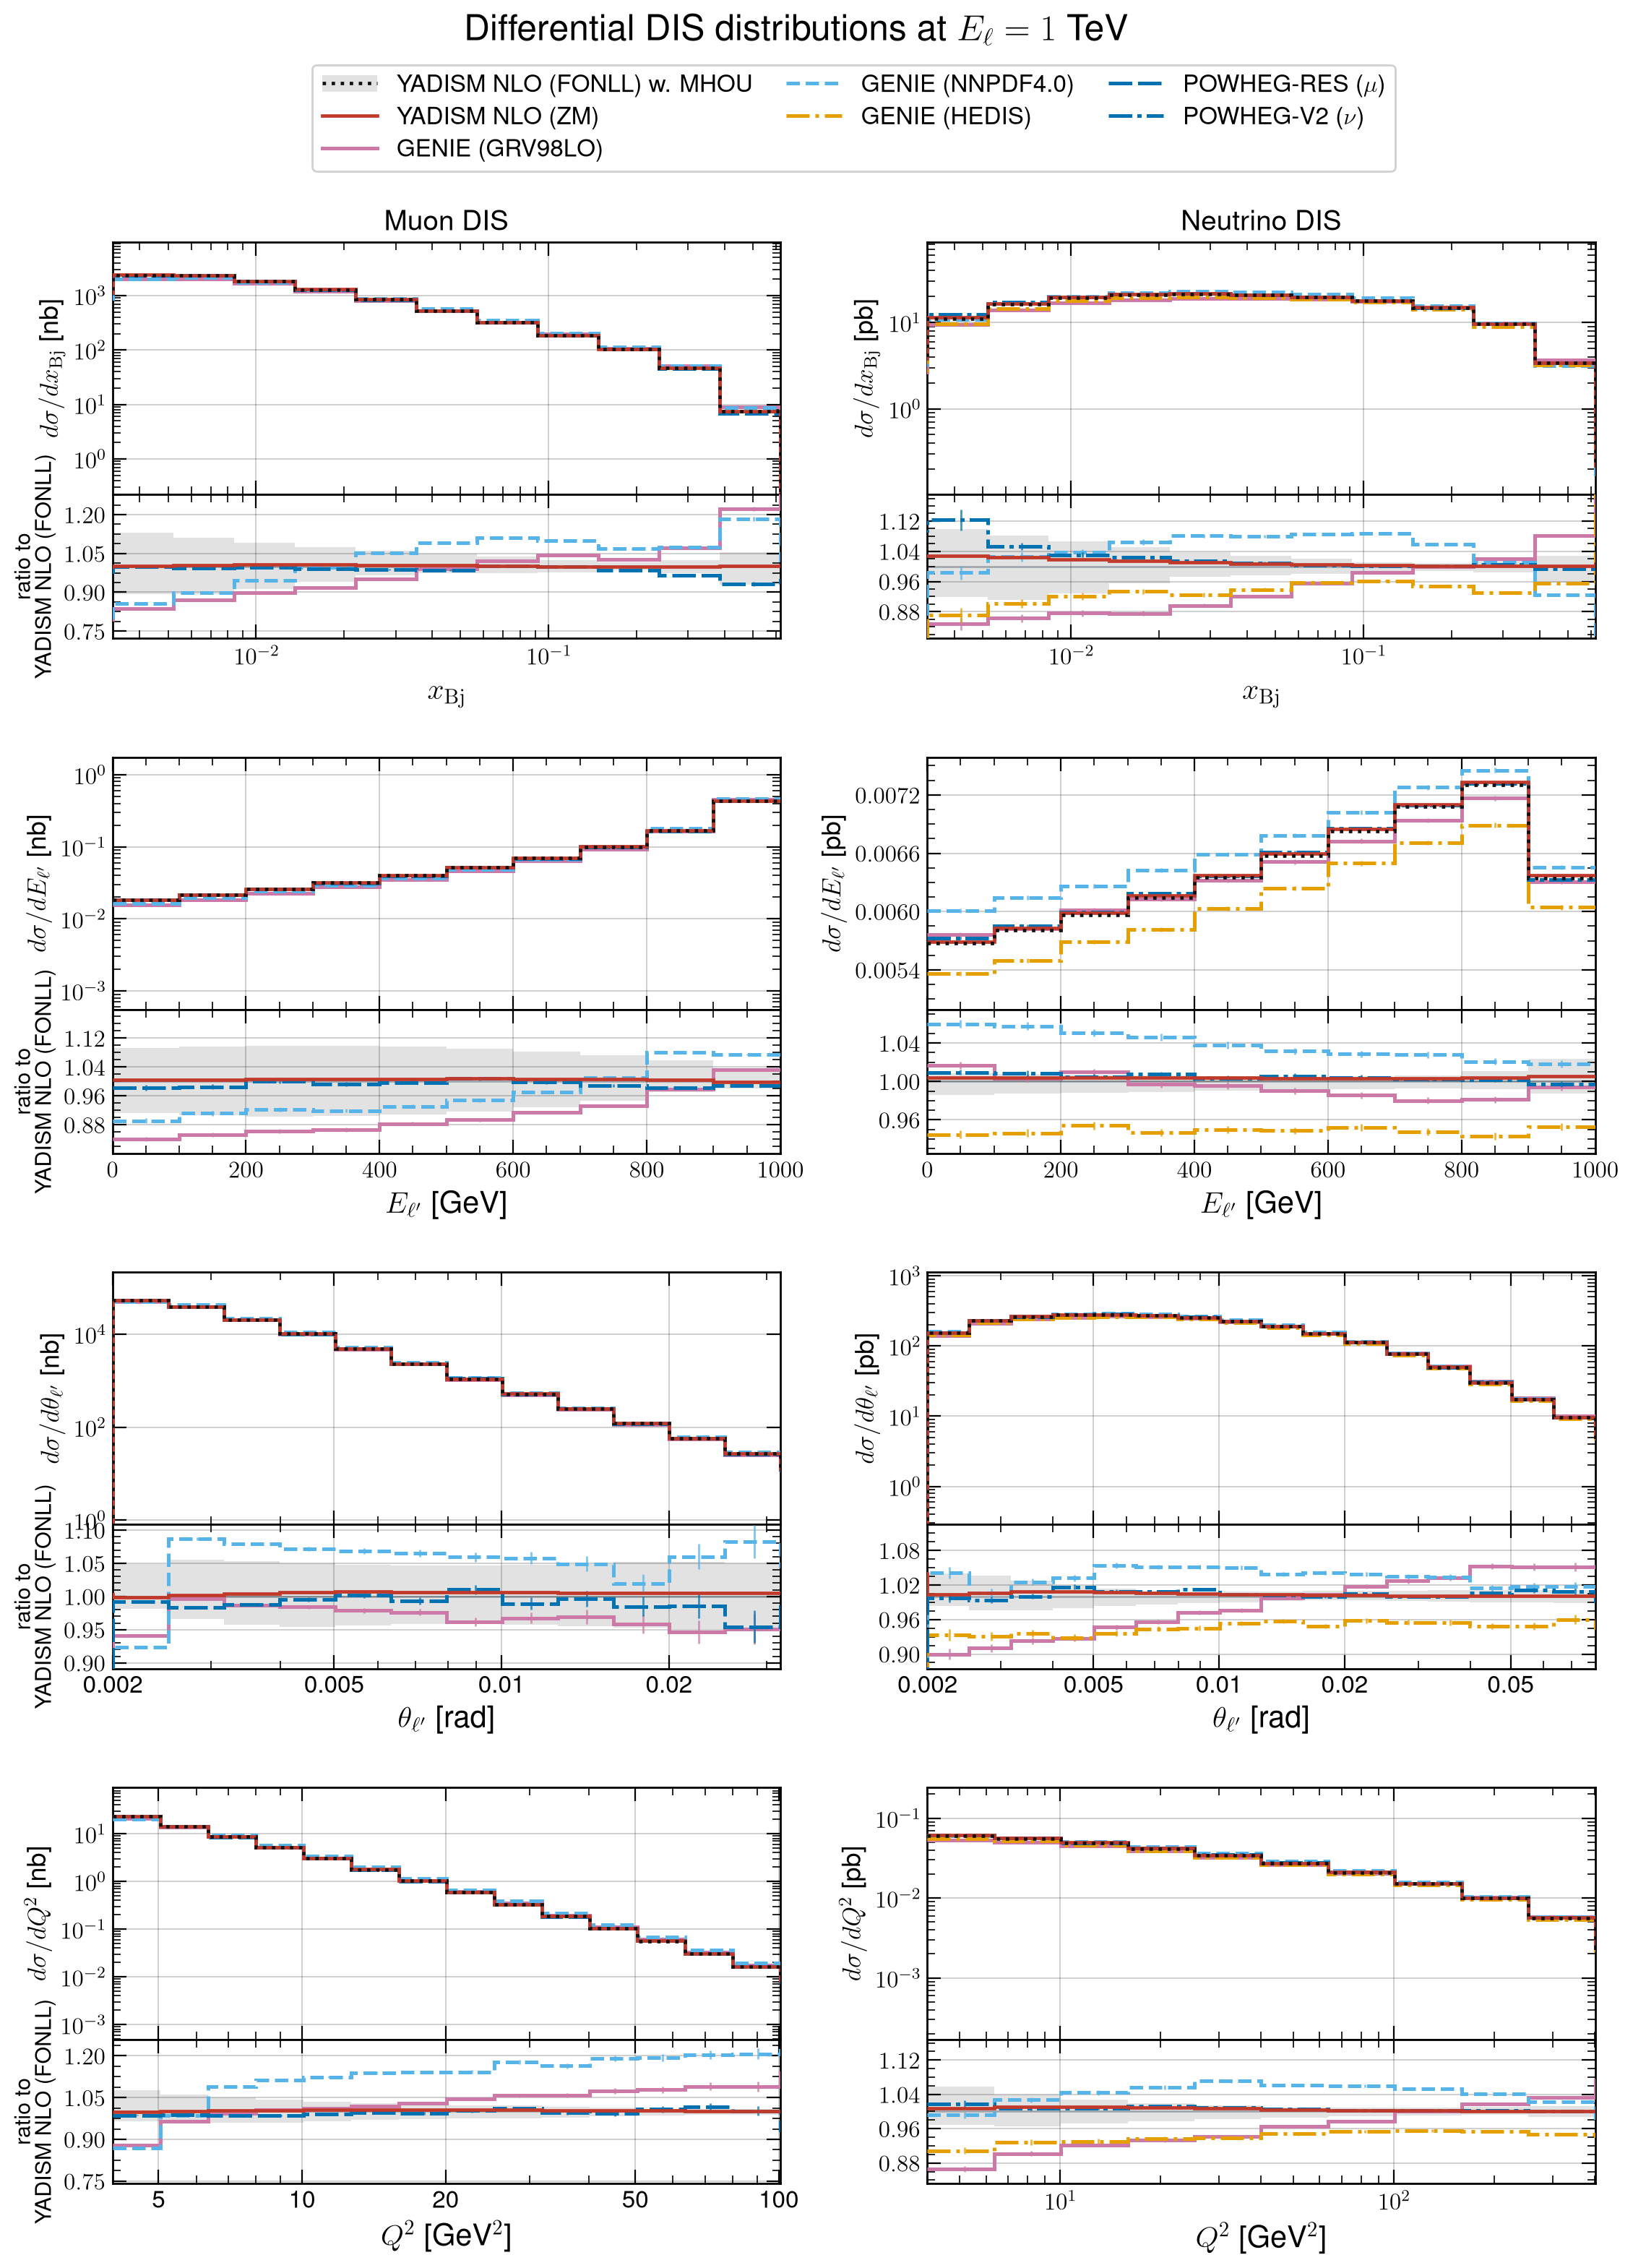
\includegraphics[width=0.96\textwidth]{figures/pp_genie_dis_distributions.png}
  \caption{\small Same as Fig.~\ref{fig:dis-distributions}
  now comparing the same muon and neutrino DIS calculations of Fig.~\ref{fig:genie-vs-energy}.
  %
  See text for more details. 
}
  \label{fig:genie-dis-distributions}
\end{figure}
%%%%%%%%%%%%%%%%%%%%%%%%%%%%

